\section{Related Work}
\label{sec:related_work}

\begin{figure*}[t]
\centering
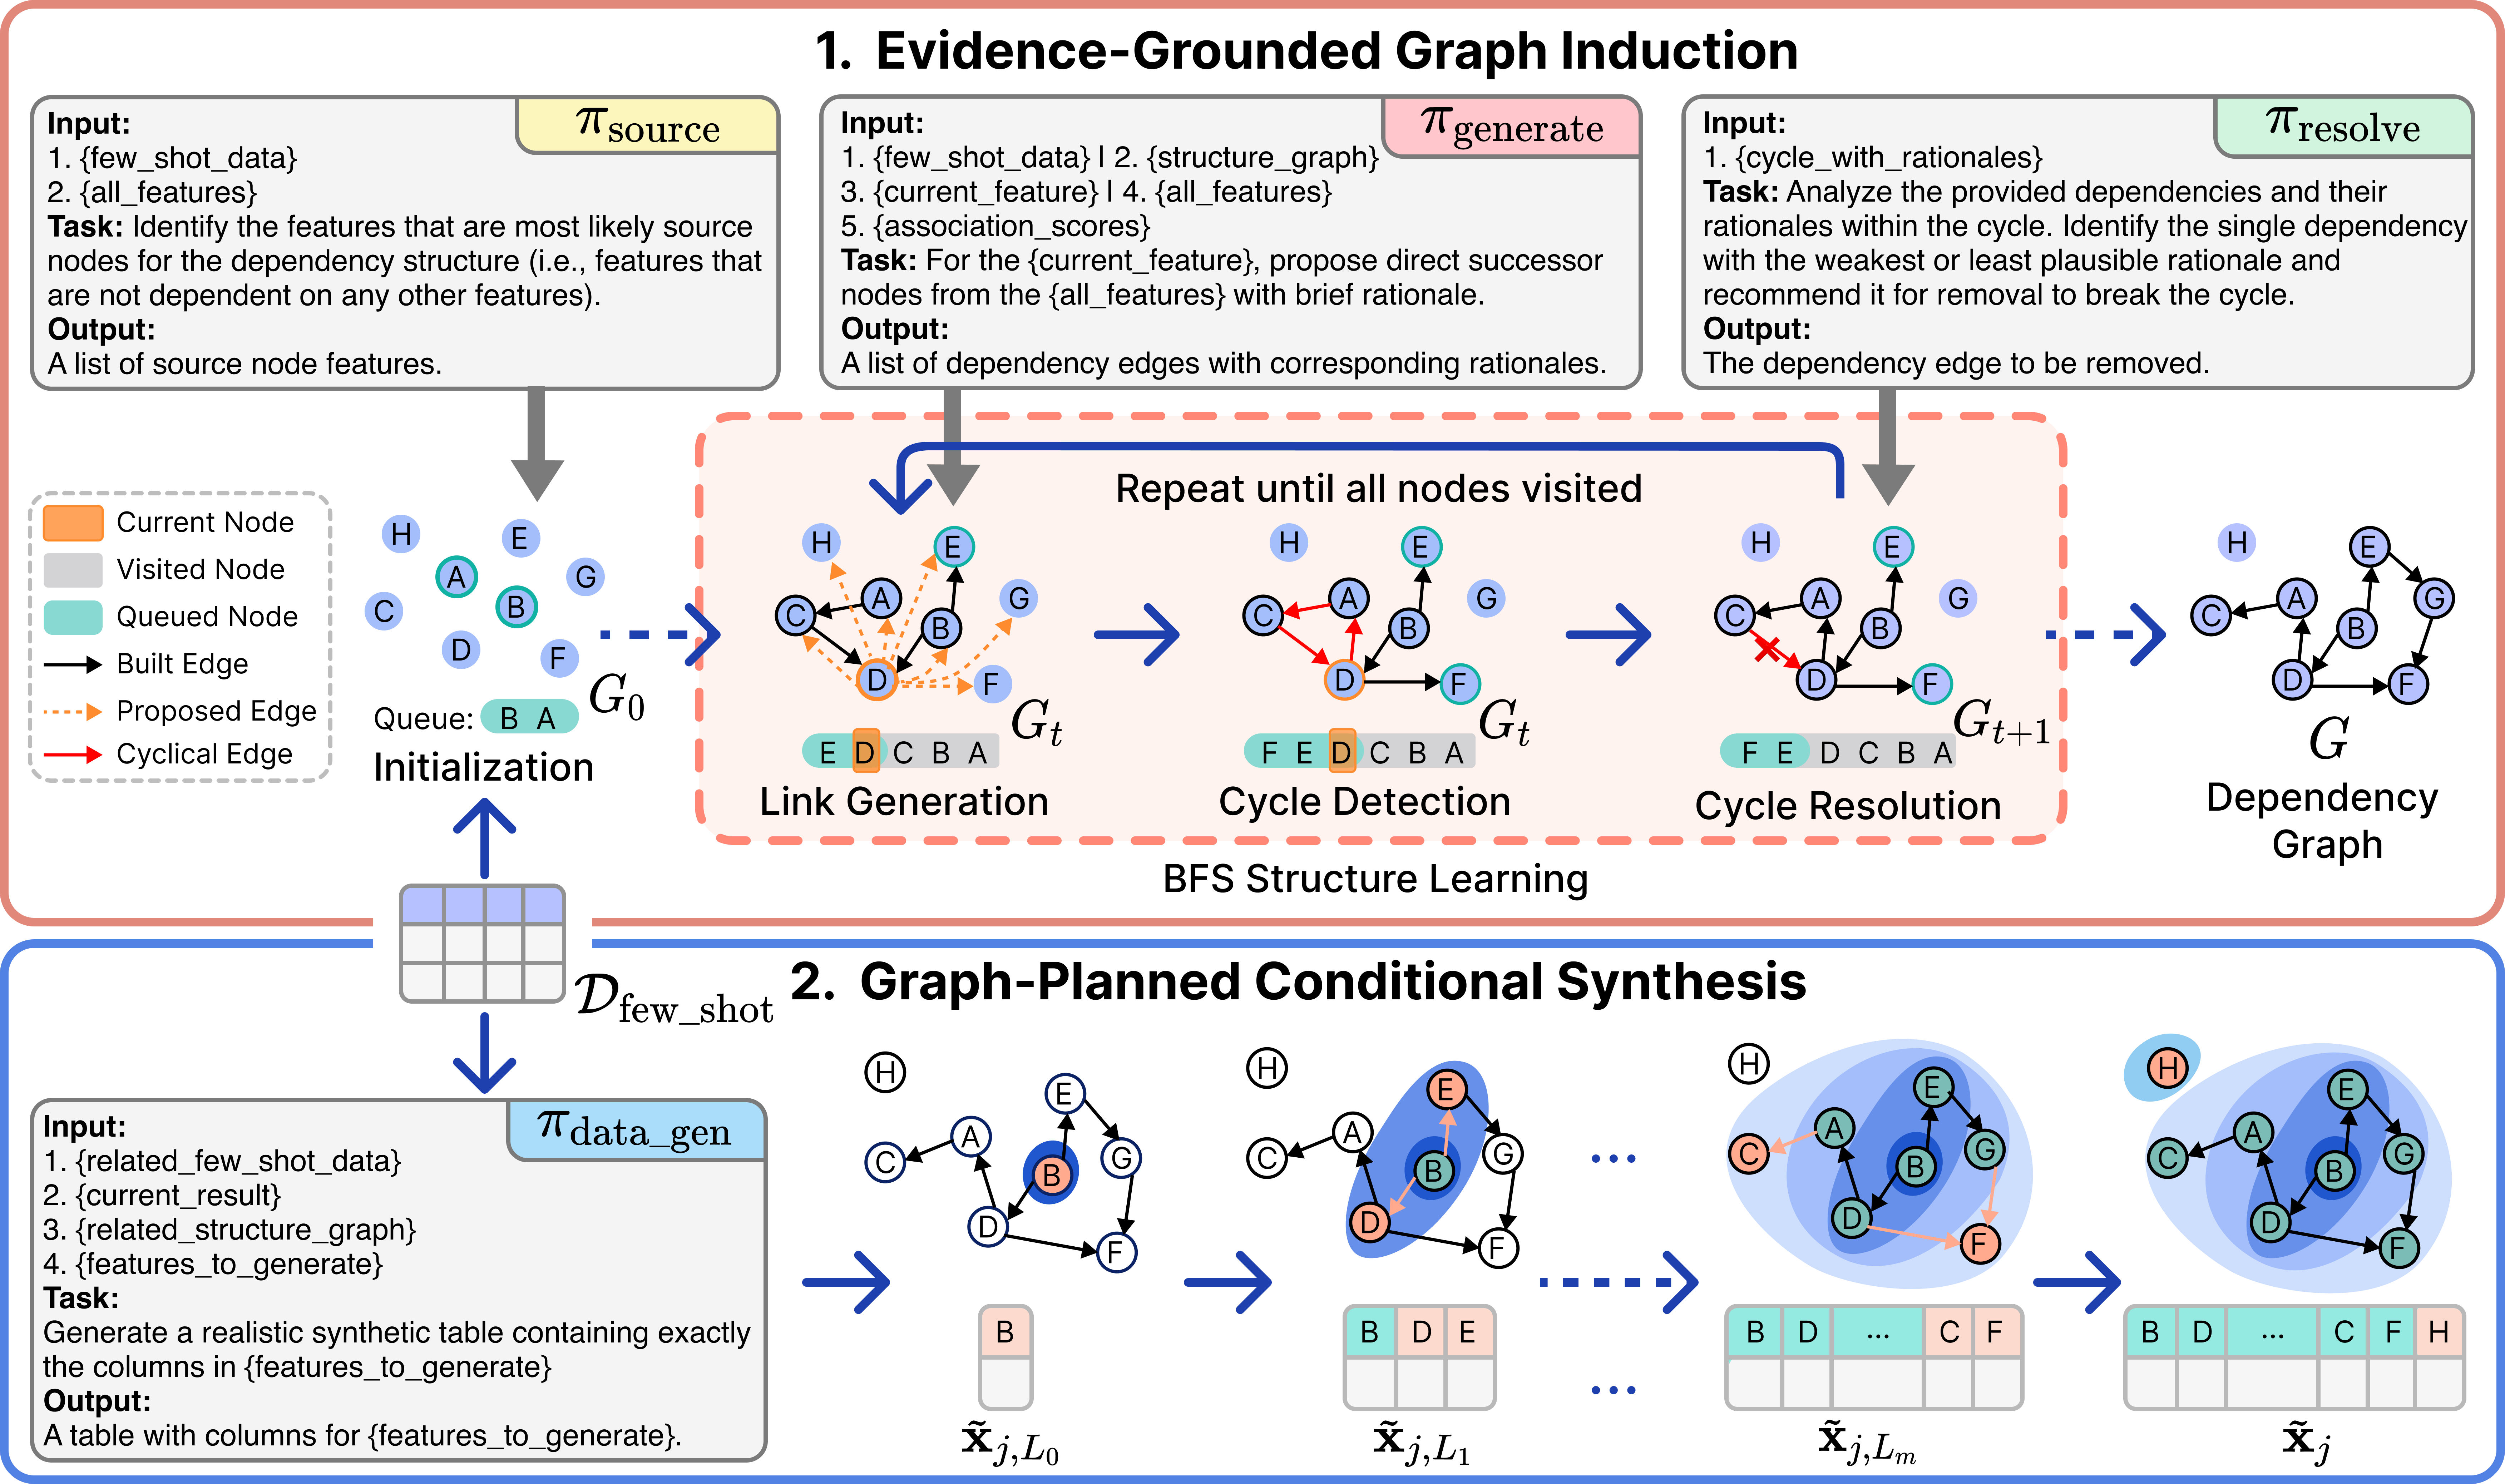
\includegraphics[width=\textwidth]{figures/pipeline2.png}
\caption{Overview of the \textsf{StructSynth} framework. The method first performs \textbf{Evidence-Grounded Graph Induction} to infer a dependency graph from limited data via an LLM-guided search. Subsequently, \textbf{Graph-Planned Conditional Synthesis} uses the learned graph as a generation plan to autoregressively guide the LLM in generating new tabular data.}
\label{fig:pipeline}
\end{figure*}

\paragraph{Tabular Synthesis in Low-Data Regimes.}
Deep generative models---including VAE-based~\cite{patki2016synthetic}, GAN-based~\cite{xu2019modeling}, and diffusion-based~\cite{kotelnikov2023tabddpm, tabsyn} approaches---capture the joint distribution end-to-end but are data-hungry and provide limited control over inter-feature dependencies.
Structure-aware methods address this by incorporating explicit dependency graphs; Bayesian-network-based generators~\cite{ankan2015pgmpy, zhang2017privbayes} and graph-based VAEs~\cite{van2021decaf, liu2023goggle} condition synthesis on learned graphical structures, yet their effectiveness degrades when the underlying graphs cannot be reliably estimated from scarce samples.


\paragraph{LLM-Based Tabular Generation.}
Fine-tuning approaches such as GReaT~\cite{borisov2023language} and TAPTAP~\cite{zhang2023generative} serialize rows as text and train LLMs for autoregressive generation, but are computationally expensive and degrade under data scarcity.
Prompt-based methods avoid parameter updates, relying instead on inference-time prompts or example selection: CuratedLLM (CLLM)~\cite{cllm2024} selects curated in-context examples to guide generation, yet does not explicitly model inter-feature dependency structure; TabGen-ICL~\cite{fang-etal-2025-tabgen} iteratively refines in-context selection to align the generated distribution with the real one.
\textcolor{blue}{PAFT~\cite{xu2024why} and GraDe~\cite{zhang-etal-2025-features} are structure-aware fine-tuning methods. PAFT compiles discovered functional dependencies into feature orders for permutation-aware fine-tuning, while GraDe combines FD-guided dynamic sparse attention with an FD-alignment objective during GPT-2 fine-tuning. Both tightly couple structure discovery with the generation model itself. \textsf{StructSynth} instead treats the graph as an inference-time \textit{generation plan} for a black-box LLM, without parameter updates.}
SPADA~\cite{yang2025doubling} further decouples the two stages by replacing LLM-based generation with lightweight statistical estimators (KDE, normalizing flows), greatly accelerating sampling but relying on sufficient data to fit reliable conditional distributions.

\paragraph{LLM-Assisted Dependency Discovery.}
LLMs have been applied to structure learning itself. Early work demonstrated that LLMs can accurately judge pairwise causal directions from variable semantics alone~\cite{kiciman2023causal}. To scale beyond pairwise queries, BFS-based strategies reframe structure discovery as a graph traversal task, substantially reducing the number of LLM calls~\cite{jiralerspong2024efficient, zanna2025fairness}. A complementary line integrates LLM judgments with classical constraint-based algorithms, using the LLM to validate or correct statistically proposed edges~\cite{ban2023causal}.
However, these methods target causal graph identification as an end in itself and do not connect the discovered structure to a downstream data generation process.
An extended discussion of all the above lines of work is provided in Appendix~\ref{app:extended_related_work}.
